% AUTO-GENERATED by `python -m analysis.results` — do not edit by hand.
\documentclass[tikz,border=2pt]{standalone}
\usepackage{pgfplots}
\pgfplotsset{compat=1.17}
\begin{document}
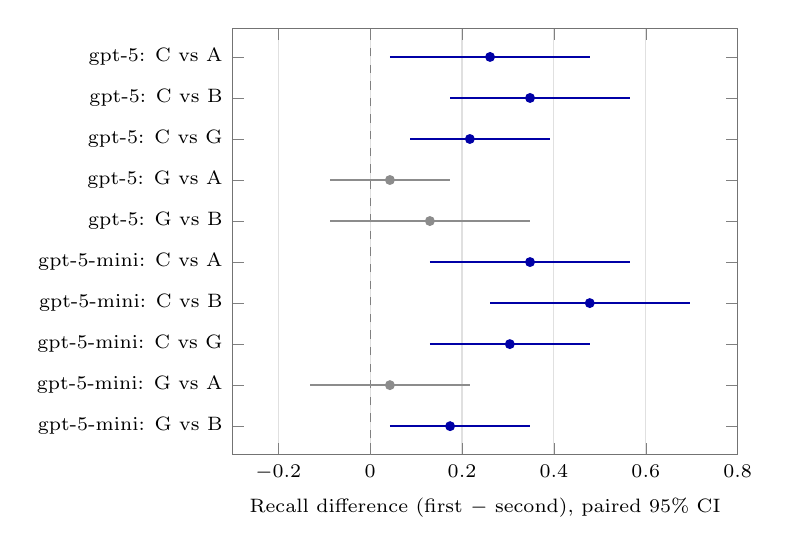
\begin{tikzpicture}[font=\footnotesize]
\begin{axis}[
  width=8cm, height=7cm, xmin=-0.3, xmax=0.8,
  ymin=-0.7, ymax=9.7, ytick={0,1,2,3,4,5,6,7,8,9},
  yticklabels={gpt-5-mini: G vs B,gpt-5-mini: G vs A,gpt-5-mini: C vs G,gpt-5-mini: C vs B,gpt-5-mini: C vs A,gpt-5: G vs B,gpt-5: G vs A,gpt-5: C vs G,gpt-5: C vs B,gpt-5: C vs A},
  xlabel={Recall difference (first $-$ second), paired 95\% CI},
  tick label style={font=\scriptsize}, label style={font=\scriptsize},
  xmajorgrids, major grid style={draw=black!12}, axis line style={black!55},
]
\draw[black!50, dashed] (axis cs:0,-0.7) -- (axis cs:0,9.7);
\draw[blue!65!black, thick] (axis cs:0.043,0) -- (axis cs:0.348,0);
\fill[blue!65!black] (axis cs:0.174,0) circle (1.8pt);
\draw[black!45, thick] (axis cs:-0.130,1) -- (axis cs:0.217,1);
\fill[black!45] (axis cs:0.043,1) circle (1.8pt);
\draw[blue!65!black, thick] (axis cs:0.130,2) -- (axis cs:0.478,2);
\fill[blue!65!black] (axis cs:0.304,2) circle (1.8pt);
\draw[blue!65!black, thick] (axis cs:0.261,3) -- (axis cs:0.696,3);
\fill[blue!65!black] (axis cs:0.478,3) circle (1.8pt);
\draw[blue!65!black, thick] (axis cs:0.130,4) -- (axis cs:0.565,4);
\fill[blue!65!black] (axis cs:0.348,4) circle (1.8pt);
\draw[black!45, thick] (axis cs:-0.087,5) -- (axis cs:0.348,5);
\fill[black!45] (axis cs:0.130,5) circle (1.8pt);
\draw[black!45, thick] (axis cs:-0.087,6) -- (axis cs:0.174,6);
\fill[black!45] (axis cs:0.043,6) circle (1.8pt);
\draw[blue!65!black, thick] (axis cs:0.087,7) -- (axis cs:0.391,7);
\fill[blue!65!black] (axis cs:0.217,7) circle (1.8pt);
\draw[blue!65!black, thick] (axis cs:0.174,8) -- (axis cs:0.565,8);
\fill[blue!65!black] (axis cs:0.348,8) circle (1.8pt);
\draw[blue!65!black, thick] (axis cs:0.043,9) -- (axis cs:0.478,9);
\fill[blue!65!black] (axis cs:0.261,9) circle (1.8pt);
\end{axis}
\end{tikzpicture}
\end{document}
